
\chapter{Week 9 -- SOH Estimation}

\section{Abstract}
This report presents an implementation of a dual-Extended Kalman Filter architecture used for state of health ($SoH$) estimation. An EKF for $SoC$ estimation using measured terminal voltage presented in the previous lab report is complemented by a second two-state EKF used for the estimation of battery capacity $C$ used to assess the state of health.

\section{Model implementation}
\label{sec:9-one}

The $SoH$ estimation architecture requires two separate models -- the battery and the slow aging process.
Just like in the previous assignment, the battery model was chosen as the standard 2RC equivalent circuit model
\begin{align}
        \dot{U_1} &= -\frac{1}{R_1 C_1} U_1 + \frac{1}{C_1} i, \label{eq:9-cont1} \\
        \dot{U_2} &= -\frac{1}{R_2 C_2} U_2 + \frac{1}{C_2} i, \\
        \dot{SoC} &= -\frac{100}{C} i, \\
        \Ubat &= \OCV(SoC) - U_1 - U_2 - R_0i,
    \label{eq:9-cont4}
\end{align}
with a nonlinear output equation, where the system input $i$ denotes the flowing current, states $U_1$ and $U_2$ are voltage drops across the two RC elements, $SoC \in \left[0, 100\right]$ \% is the state of charge, $\Ubat$ is the battery terminal voltage (system output) and the open circuit voltage $\OCV(SoC)$, resistances $R_{0,1,2}$ and capacitances $C_{1,2}$ are (possibly $SoC$-dependent) model parameters with numeric values provided as a part of the assignment. In this task the total capacity $C$ is not assumed constant and is estimated by the second EKF.
To facilitate a simple iterative simulation of system behavior, the system \eqref{eq:9-cont1}-\eqref{eq:9-cont4} was discretized using the Forward Euler method as
\begin{equation}
\begin{split}
    x(k+1) &= x(k) + T_s f(x(k), u(k)), \\
    y(k) &= g(x(k), u(k)),
\end{split}
\label{eq:9-disc}
\end{equation}
where $f$ and $g$ are vector functions of right-hand sides of \eqref{eq:9-cont1}-\eqref{eq:9-cont4} and $x(k)$, $u(k)$ and $y(k)$ are the system state, input and output vector at sample $k$, respectively.

Battery ageing is modelled as a gradual decrease of the available capacity $C$. There are no degradation dynamics modelled
\begin{align}
    C(k+1) &= C(k) + v_1(k), \\
    \hat{SoC}(k+1) &= \hat{SoC}(k) - \frac{1}{C(k)}i(k) + v_2(k),
\end{align}
hence any change in the battery capacity $C$ originates from the influence of process noise $v(k)$. The quantity $\hat{SoC}$ is a secondary estimate of battery $SoC$ calculated by the SoH-EKF. It acts as an output of the SoH-EKF that is compared to the $SoC$ estimate given by SoC-EKF to obtain the prediction error. This prediction error then drives the SoH-EKF to estimate the correct battery capacity.
\clearpage
\section{Experimental results}

Equations were implemented in code to verify that the model and provided parameters work correctly and can reproduce the reference waveforms. A comparison of reference (given) and my simulated signals is in Fig. \ref{fig:9-validation}. Signals clearly do not match, indicating a significant discrepancy in the provided model and model used to generate reference data.
Although many iterations of the trial and error method showed that part of the discrepancy is caused by the neglected Coulombic efficiency $\eta \approx 0.977$, it is not the only cause. It is -- for example -- not clear from the assignment, where in the cycle is the reference battery capacity (recorded as one sample per charge-discharge cycle) recorded. Apart from that, it is unspecified whether the capacity in the reference simulation is piecewise constant or linearly decreasing during the cycle. These uncertainties about the provided data result in significant errors in the result.


\begin{figure}[hbp]
    \centering
\begin{subfigure}{0.49\textwidth}
    \centering
    \includegraphics[width=\textwidth]{figures/9/validation-soc.eps}
    \caption{State of charge $SoC$.}
    \label{fig:9-validation-SOC}
    \end{subfigure}
    \hfill
    \begin{subfigure}{0.49\textwidth}
    \centering
    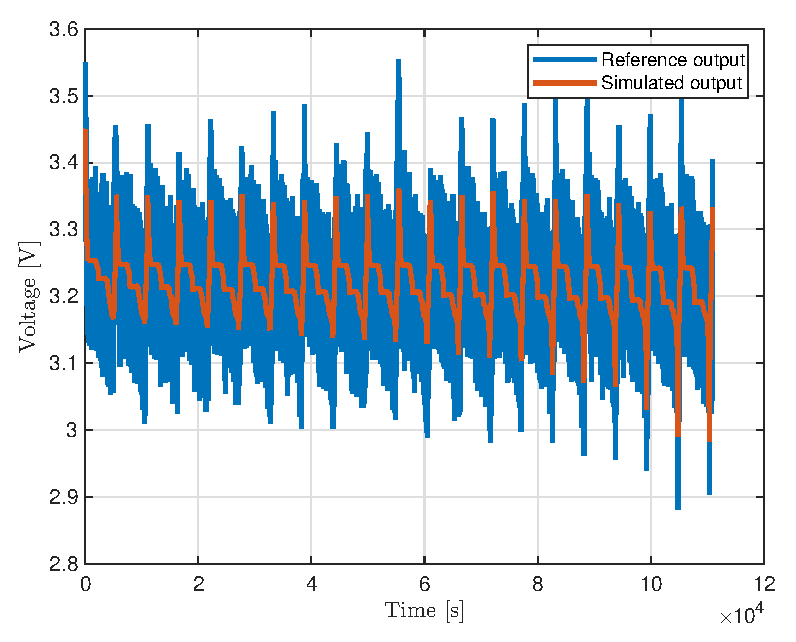
\includegraphics[width=\textwidth]{figures/9/validation-U.eps}
    \caption{Terminal voltage $\Ubat$.}
    \label{fig:9-validation-U}
    \end{subfigure}
    
    \caption{Comparison of reference and simulated waveforms.}
    \label{fig:9-validation}
\end{figure}

The dual EKF architecture was implemented regardless of the lack of information. Best results achieved using covariance matrices $\mathbf{R}_{\text{SoH}} = 1$, $\mathbf{R}_{\text{SoC}} = 0.05$, $\mathbf{Q}_{\text{SoH}} = diag(10^{-6}, 10^{-6}, 3\cdot 10^{-2})$ and $\mathbf{Q}_{\text{SoC}} = diag(10^{-8}, 10^{-10})$ are shown in Fig. \ref{fig:9-soc}. Both EKFs track the reference SoC with RMSE of 3.0 \%  over the whole experiment. The cell capacity $C$ estimated by SoH-EKF is shown in Fig. \ref{fig:9-capacity}. There is some non-negligible error (a 0.5 Ah bias) caused most probably by the mismatch of models used to generate reference data and to design the EKF. Nevertheless one can see the theoretical strenght of the dual EKF architecture for SoH estimation since the estimate capacity decreases with the same gradient as the reference.

\begin{figure}[hbp]
    \centering
\begin{subfigure}{0.49\textwidth}
    \centering
    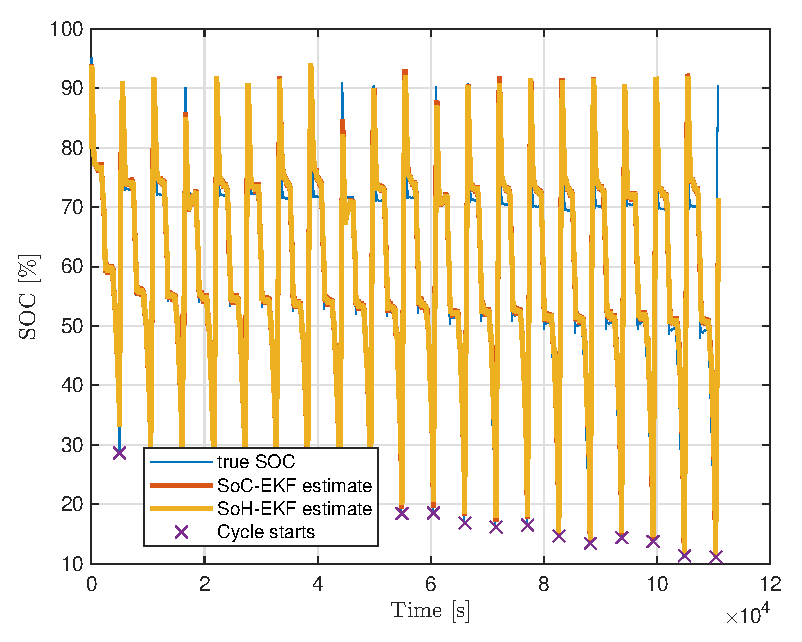
\includegraphics[width=\textwidth]{figures/9/soc-estimate.eps}
    \caption{SoC For the whole experiment.}
    \label{fig:9-soc-estimate}
    \end{subfigure}
    \hfill
    \begin{subfigure}{0.49\textwidth}
    \centering
    \includegraphics[width=\textwidth]{figures/9/soc-estimate-detail.eps}
    \caption{Detail of a single discharge-charge cycle.}
    \label{fig:9-soc-estimate-detail}
    \end{subfigure}
    
    \caption{SoC estimates given by the dual EKF architecture.}
    \label{fig:9-soc}
\end{figure}
 

\begin{figure}
    \centering
    \includegraphics{figures/9/capacity-estimate.eps}
    \caption{Estimated and reference battery capacity}
    \label{fig:9-capacity}
\end{figure}

